\documentclass[letterpaper,10pt]{article}

\usepackage{color}
\usepackage{tikz}
\usepackage{caption}

\setlength{\headheight}{0in}
\setlength{\marginparsep}{0in}
\setlength{\footskip}{0in}
\setlength{\headsep}{0in}
\setlength{\marginparwidth}{0in}
\setlength{\marginparpush}{0in}
\setlength{\voffset}{0in}
\setlength{\hoffset}{-1in}
\setlength{\voffset}{-1in}
\setlength{\oddsidemargin}{0.75in}
\setlength{\evensidemargin}{0.75in}
\setlength{\topmargin}{0.75in}
\setlength{\textheight}{9.5in}
\setlength{\textwidth}{7in}
\setlength{\parindent}{0in}
\setlength{\parskip}{10pt} %change this to match font size

\pagestyle{empty}
\definecolor{gray}{gray}{0.75}
\usetikzlibrary{shapes,arrows,calc}

% define block styles
\tikzstyle{line} = [draw, -latex']
\tikzstyle{block} = [draw, rectangle, text centered, minimum height=2em]
\tikzstyle{mlblock} = [draw, rectangle, text width=10em, text centered, minimum height=2em]
\tikzstyle{decision} = [draw, diamond, text width=4.5em, text centered, node distance=3cm, inner sep=0pt]
\tikzstyle{cloud} = [draw, rectangle, text centered, rounded corners, minimum height=2em]

\begin{document}
    Albert Chang and Nipun Chopra\\
    CSE-380 A6\\
    University at Buffalo\\
    Dr. Kris Schindler\\
    March 22, 2011\\
    \textit{Lab 6 Documentation}

    The objective of Lab 6 was to learn how to use the 32-bit timer. A curses-like
    environment is output to the terminal, with an asterisk bouncing back and
    forth. With the keyboard, the user can adjust the speed of the asterisk, and
    can pause it. All of this is accomplished with interrupts.

    The following routines were imported through the \textit{library.s} file:
    \textit{uart\_init}, \textit{output\_character}, \textit{read\_character},
    and \textit{output\_string}. Figs. \ref{flo:uart_init},
    \ref{flo:io_char}, and \ref{flo:output_string} are their respective
    flowcharts for each routine. The only change to \textit{uart\_init} was to
    set the baud rate to 1152000 so there wouldn't be any flickering when it
    refreshed. It still flickers when the asterisk is moving too fast.

    \begin{figure}[h]
        \begin{center}
    \begin{tikzpicture}[node distance = 3cm, auto]
        \node[cloud] (origin) {Start};
        \node[block, below of=origin, node distance=1.5cm] (enable) {Write 0x5 to PINSEL0 to enable UART0};
        \node[mlblock, below of=enable] (init) {Configure U0LCR:\\%
                                                8-bit word length\\%
                                                1 stop bit\\%
                                                no parity\\%
                                                disable break control\\%
                                                enable access latch};
        \node[block, below of=init] (baud) {Set baud rate to 9600};
        \node[mlblock, below of=baud] (conf) {Configure U0LCR:\\%
                                                8-bit word length\\%
                                                1 stop bit\\%
                                                no parity\\%
                                                disable break control\\%
                                                disable latch access};
        \node[cloud, below of=conf] (stop) {Stop};
        \path[line] (origin) -- (enable);
        \path[line] (enable) -- (init);
        \path[line] (init) -- (baud);
        \path[line] (baud) -- (conf);
        \path[line] (conf) -- (stop);
    \end{tikzpicture}
\end{center}

        \caption{Flowchart of \textit{uart\_init} routine.}
        \label{flo:uart_init}
    \end{figure}

    \begin{figure}[h]
        \begin{minipage}{0.5\linewidth}
            \begin{center}
    \begin{tikzpicture}[node distance = 1.5cm, auto]
        \node[cloud] (origin) {Start};
        \node[decision, below of=origin] (test) {Test THRE in status register};
        \node[block, below of=test, node distance = 3.5cm] (store) {Store byte in transmit register};
        \node[cloud, below of=store] (stop) {Stop};
        \path[line] (origin) -- (test);
        \path[line] (test) -- node [near start] {1} (store);
        \path[line] (test) -| node [near start] {0} +(3,2.25) -- +(0,2.25);
        \path[line] (store) -- (stop);
    \end{tikzpicture}
\end{center}

        \end{minipage}%
        \begin{minipage}{0.5\linewidth}
            \begin{center}
    \begin{tikzpicture}[node distance = 1.5cm, auto]
        \node[cloud] (origin) {Start};
        \node[decision, below of=origin] (test) {Test RDR in status register};
        \node[block, below of=test, node distance = 3.5cm] (read) {Read byte from receive register};
        \node[cloud, below of=read] (stop) {Stop};
        \path[line] (origin) -- (test);
        \path[line] (test) -- node [near start] {1} (read);
        \path[line] (test) -| node [near start] {0} +(3,2) -- +(0,2);
        \path[line] (read) -- (stop);
    \end{tikzpicture}
\end{center}

        \end{minipage}
        \caption{Flowcharts of \textit{output\_character} (left) and \textit{read\_character} (right) routines.}
        \label{flo:io_char}
    \end{figure}

    \begin{figure}[h]
        \begin{center}
    \begin{tikzpicture}[node distance = 1.5cm, auto]
        \node[cloud] (origin) {Start};
        \node[block, below of=origin] (read) {Load byte from memory};
        \node[decision, below of=read] (null) {Is it the null character?};
        \node[block, right of=null, node distance=5cm] (output) {Output character};
        \node[cloud, below of=null, node distance=3cm] (stop) {Stop};
        \path[line] (origin) -- (read);
        \path[line] (read) -- (null);
        \path[line] (null) -- node [near start] {no} (output);
        \path[line] (output) |- (read);
        \path[line] (null) -- node [near start] {yes} (stop);
    \end{tikzpicture}
\end{center}

        \caption{Flowchart of \textit{output\_string} routine.}
        \label{flo:output_string}
    \end{figure}

    \clearpage

    Just as with the previous lab, the main routine, \textit{lab6}, doesn't do
    much besides call upon the initialization routines, \textit{uart\_init} and
    \textit{interrupt\_init}. Afterwards it sets up the initial speed of the
    asterisk, provides the initial output, and starts the timer. The output is
    only changed when something has changed, instead of every cycle. Changes
    are only made when the timer count register matches the match register.

    \begin{minipage}{\linewidth}
        \begin{center}
    \begin{tikzpicture}[node distance=1.5cm, auto]
        \node[cloud] (origin) {Start};
        \node[block, below of=origin] (uart) {Initialize UART0};
        \node[block, below of=uart] (interrupt) {Initialize interrupts};
        \node[block, below of=interrupt] (speed) {Setup initial speed};
        \node[block, below of=speed] (output) {Initial output};
        \node[block, below of=output] (time) {Start timer};
        \node[cloud, below of=time] (stop) {Stop};
        \path[line] (origin) -- (uart);
        \path[line] (uart) -- (interrupt);
        \path[line] (interrupt) -- (speed);
        \path[line] (speed) -- (output);
        \path[line] (output) -- (time);
        \path[line] (time) -- (stop);
    \end{tikzpicture}
\end{center}

        \captionof{figure}{Flowchart of \textit{lab6} routine.}
        \label{flo:main}
    \end{minipage}

    The \textit{interrupt\_init} routine is similar to the previous lab's,
    except instead of enabling and configuring the external interrupt, it
    enables and configures timer interrupt.

    \begin{minipage}{\linewidth}
        \begin{center}
    \begin{tikzpicture}[node distance=1.5cm, auto]
        \node[cloud] (origin) {Start};
        \node[block, below of=origin] (gpio) {Enable push button};
        \node[block, below of=gpio] (classify) {Classify push button and UART0 as FIQ};
        \node[block, below of=classify] (enable) {Enable interrupts};
        \node[block, below of=enable] (edge) {Setup up external interrupt 1 as edge sensitive};
        \node[block, below of=edge] (uart) {Setup UART0 interrupt on RBR fill};
        \node[block, below of=uart] (fiq) {Enable fast interrupts, disable normal interrupts};
        \node[cloud, below of=fiq] (stop) {Stop};
        \path[line] (origin) -- (gpio);
        \path[line] (gpio) -- (classify);
        \path[line] (classify) -- (enable);
        \path[line] (enable) -- (edge);
        \path[line] (edge) -- (uart);
        \path[line] (uart) -- (fiq);
        \path[line] (fiq) -- (stop);
    \end{tikzpicture}
\end{center}

        \captionof{figure}{Flowchart of \textit{interrupt\_init} routine.}
        \label{flo:interrupt_init}
    \end{minipage}

    Again, the bulk of the program is handled by the fast interrupt handler,
    \textit{FIQ\_Handler}. Depending on which kind of interrupt it is, it takes
    the appropriate action.

    \begin{center}
    \begin{tikzpicture}[node distance=1.5cm, auto]
        \node[cloud] (origin) {Start};
        \node[decision, below of=origin] (timer) {Interrupt caused by timer?};
        \node[block, below of=timer, node distance=3cm] (uninter) {Reset timer interrupt};
        \node[block, below of=uninter] (formfeed) {Clear terminal};
        \node[block, below of=formfeed] (topout) {Output top portion};
        \node[block, below of=topout] (get) {Get position and direction};
        \node[block, below of=get] (update) {Update position, change position if necessary};
        \node[block, below of=update] (term) {Update terminal output};
        \node[block, below of=term] (set) {Save position and direction};
        \node[block, below of=set] (botout) {Output bottom portion};
        \node[decision, below of=botout] (uart) {Interrupt caused by UART?};
        \node[block, below of=uart, node distance=3cm] (read) {Read input};
        \path[line] (origin) -- (timer);
        \path[line] (timer) -- node [near start] {yes} (uninter);
        \path[line] (uninter) -- (formfeed);
        \path[line] (formfeed) -- (topout);
        \path[line] (topout) -- (get);
        \path[line] (get) -- (update);
        \path[line] (update) -- (term);
        \path[line] (term) -- (set);
        \path[line] (set) -- (botout);
        \path[line] (botout) -- (uart);
        \path[line] (uart) -- node [near start] {yes} (read);
        \path[line, dotted] (read) -- +(0,-1.5);
        \path[line] (timer) -| node [near start] {no} +(-7.5,-16.5) -- (uart);
        \draw (uart) -| node [near start] {no} +(7.5,-3);
        \path[line, dotted] (uart) +(7.5,-3) -- +(7.5,-4.5);
    \end{tikzpicture}
\end{center}


    \begin{minipage}{\linewidth}
        \begin{center}
    \begin{tikzpicture}[node distance=1.5cm, auto]
        \node[decision] (paused) {Was the space bar hit?};
        \node[block] at +(-4.5,-3) (rst) {Reset and stop timer counter};
        \node[block, below of=rst] (get) {Get Speed and saved speed information};
        \node[decision, below of=get] (plus) {Did the user hit '+'?};
        \node[block, below of=plus, node distance=3cm] (inc) {LSR speed, restore any bit pushed off};
        \node[decision, below of=inc] (minus) {Did the user hit '-'?};
        \node[block, below of=minus, node distance=3cm] (dec) {LSL speed, save bit pushed off};
        \node[block, below of=dec] (set) {Set speed and store bits pushed off};
        \node[block, below of=set] (strt) {Start timer};
        \node[block, right of=rst, node distance=7.5cm] (toggle) {Toggle disable/enable bit in TCR};
        \node[cloud, below of=paused, node distance=21cm] (stop) {Stop};
        \path[line, dotted] (paused) +(0,3) -- (paused);
        \draw[dotted] (paused) +(7.5,3) -- +(7.5,0);
        \path[line] (paused) +(7.5,0) |- (stop);
        \draw (toggle) -- +(4.5,0);
        \path[line] (paused) -| node [near start] {no} (rst);
        \path[line] (rst) -- (get);
        \path[line] (get) -- (plus);
        \path[line] (plus) -- node [near start] {yes} (inc);
        \path[line] (inc) -- (minus);
        \path[line] (minus) -- node [near start] {yes} (dec);
        \path[line] (dec) -- (set);
        \path[line] (set) -- (strt);
        \path[line] (strt) |- (stop);
        \path[line] (paused) -| node [near start] {yes} (toggle);
        \path[line] (plus) -| node [near start] {no} +(-4.5,-6) -- (minus);
        \path[line] (minus) -| node [near start] {no} +(4.5,-4.5) -- (set);
    \end{tikzpicture}
\end{center}

        \captionof{figure}{Flowchart of \textit{FIQ\_Handler} routine.}
        \label{flo:fiq_handler}
    \end{minipage}

    There wasn't really a clear distribution of labor. It was all programmed in
    one lab session via pair programming.

\end{document}
